\documentclass[12pt]{article}
% Tickz to draw block scheme


\usepackage{verbatim}




\def\uu#1{\underline{\underline{#1}}}
\newcommand*{\rom}[1]{\expandafter\@slowromancap\romannumeral #1@}
\usepackage{amsmath}
\usepackage{resizegather}


%\newcommand{\bibfont}{\footnotesize}

\linespread{1.0}




%%%%%%%%%%%%%%%%%%%%%%%%%%%%%%%%%%%%%%%%%%%%%%%%%%%%%%%%%%%%%%%%%%%%%%%%%%%%%%%%%%%%%%%%%%%%%%%%%%%%%%%%%%%%%%% begin[document]
\begin{document}
\title{\textbf{Introducing Correlation among subcarriers\\}}
\author{Sidney Golstein}
\maketitle



%%%%%%%%%%%%%%%%%%%%%%%%%%%%%%%%%%%%%%%%%%%%%%%%%%%%%%%%%%%%%%%%%%%%%%%%%%%%%%%%%%%%%%%%%%%%%%%%%%%%%%%%%%%%% abstract
\section{Short Reminder}
We consider that we have $Q$ channel subcarriers, that we spread (via $\spread$) our symbols  $\textbf{x}$ by a factor $U$ called back-off rate (BOR). We send $N = Q/U$ symbols per OFDM block. At the transmitter side, we precode the data by the complex conjugate version of Bob's channel frequency response ($\HB^H$). We add an artifical noise signal ($\textbf{w}$) which lies in Bob null space, i.e., $\spread^H \HB \textbf{w} = \textbf{0}$. At the receiver side, we despread the received sequence at Bob via $\spread^H$, and we decode the received sequence with a particular decoding structure $\textbf{G}$ at Eve. The communication scheme is presented below:

\tikzstyle{block} = [draw, fill=gray!20, rectangle, 
minimum height=2em, minimum width=2.5em]
\tikzstyle{sum} = [draw, fill=gray!20, circle, node distance=.1cm,inner sep=0pt]
\tikzstyle{input} = [coordinate]
\tikzstyle{output} = [coordinate]
\tikzstyle{pinstyle} = [pin edge={to-,thin,black}]


\begin{tikzpicture}[auto, node distance=2cm,>=latex']
\label{TR_secure}
% We start by placing the blocks
\node [input, name=symbol] {};
\node [block, right of=symbol] (spreading) {\footnotesize Spreading : $\spread$};
\node [block, right of=spreading, node distance=3.5cm] (precoding){\footnotesize Precoding : $\HB^H$};

\node [sum, right of=precoding, pin={[pinstyle]below: \footnotesize $\textbf{w}$},
node distance=2.5cm] (sum) {\footnotesize$+$};

\node [block, right of= sum,node distance=2cm] (channel_bob) {\footnotesize $\HB$};

\node [sum, right of=channel_bob, pin={[pinstyle]below:\footnotesize $\textbf{v}_\text{B}$},
node distance=2cm] (sum2) {\footnotesize$+$};

\node [block, below of=channel_bob] (channel_eve) {\footnotesize$\HE$};

\node [sum, right of=channel_eve, pin={[pinstyle]below:$\textbf{v}_\text{E}$},
node distance=2cm] (sum3) {\footnotesize$+$};

\node [block, right of= sum2,node distance=2cm,fill=blue!20] (despread_bob) {\footnotesize $\spread^H$};

\node [block, right of= sum3,node distance=2cm,fill=red!70] (filt_eve) {\footnotesize  $\textbf{G}$};

\node [output, right of=despread_bob] (outputb) {};

\node [output, right of=filt_eve] (outpute) {};

%\node [block, right of=channel, pin={[pinstyle]above:Disturbances},
%        node distance=3cm] (system) {System};
% We draw an edge between the controller and system block to 
% calculate the coordinate u. We need it to place the measurement block. 
%\draw [->] (precoding) -- node[name=y] {$\underline{Y}$} (sum);
%\node [output, right of=system] (output) {};
%\node [block, below of=u] (measurements) {Measurements};

% Once the nodes are placed, connecting them is easy. 
\draw [draw,->] (symbol) -- node {\footnotesize$\textbf{x}$} (spreading);


\draw [->] (spreading) -- node [name = spread]{} (precoding);

\draw [->] (precoding) -- node [name = sum_an] {} (sum);
\draw [->] (sum) -- node [name = to_bob] {} (channel_bob);


\draw [->] (to_bob) |- (channel_eve);


\draw [->] (channel_bob) -- node [name = noise_bob] {} (sum2);


\draw [->] (channel_eve) -- node [name = noise_eve] {} (sum3);


\draw [->] (sum2) -- node [name = dspr_eve] {} (despread_bob);


\draw [->] (sum3) -- node [name = dspr_eve] {} (filt_eve);


\draw [draw = blue,->] (despread_bob) -- node [name = eq_bob1] {\footnotesize$\textbf{y}_{\text{B}}^{H}$} (outputb);


\draw [draw = red,->] (filt_eve) -- node [name = eq_eve1] {\footnotesize$\textbf{y}_{\text{E}}^{H}$} (outpute);
\end{tikzpicture}




%%%%%%%%%%%%%%%%
\section{Problem Statement}
We want to analyze the effect of the introduction of correlation among channel subcarriers, i.e., the effect of frequency correlation in our system. \\
In the time-domain, we modelize the channel thanks to $L$ taps:
\begin{equation}
	h = [h_1 ... h_L]^T
	\label{eq:channel_TD}
\end{equation}
The time-domain correlation function is given by:
\begin{equation}
	\EX{h h^H} := C_h(\tau) = \text{diag}(p_1 ... p_L)
	\label{eq:corr_fct_TD}
\end{equation}
where $(p_1 ... p_L) := P(\tau)$ is the power delay profile (PDP). It gives the power density (per delay unit) incident onto a local area as a function of the propagation delay $\tau$. The Fourrier transform of the PDP is the correlation function in the frequency domain:
\begin{equation}
 C_H(\Delta f) = \int_{-\infty}^{\infty} P(\tau) e^{-j 2\pi \Delta f \tau} d\tau
\label{eq:corr_fct_FD}
\end{equation}
where $\Delta f$ is the frequency difference between two particular subcarriers. The PDP $P(\tau)$ is often assumed to follow an exponential model:
\begin{equation}
	P(\tau) = P_0 \; e^{-\tau/\sigma_\tau}  \; \; , \; \tau \geq 0
	\label{eq:PDP_model}
\end{equation}
where $\sigma_\tau$ is the delay spread which characterizes the PDP duration and depends on the physical environment.\\
From (\ref{eq:corr_fct_FD}) and (\ref{eq:PDP_model}), we obtain the frequency-domain correlation function as:
\begin{equation}
	C_H(\Delta f) = \frac{P_0 \sigma_\tau}{1+ 2\pi j \sigma_\tau \Delta f}
	\label{eq:correl_fct}
\end{equation}
Another parameter that characterizes the environment is the coherence bandwidth ($\Delta f_C$) which is defined as the bandwidth over which the correlation is above a certain threshold (typically 0.7):
\begin{equation}
	\Delta f_C \approx \frac{1}{2\pi\sigma_\tau}
	\label{eq:coherence_bw}
\end{equation}
In the simulation, we consider a normalized frequency-domain correlation function, i.e. $P_0 \sigma_\tau = 1$. If we have Q channel subcarriers, we create a correlation matrix given by:
\begin{equation}
\textbf{C}_H = 
\begin{bmatrix}
	1 & c_{1,2} & \hdots & c_{1,Q}  \\
	c_{1,2}^* & 1 & \hdots & c_{2,Q} \\
	\vdots & & \ddots & \vdots \\
	c_{1,Q}^* & c_{2,Q}^* & \hdots & 1
\end{bmatrix}
\label{eq:correl_mat}
\end{equation}
where the $c_{i,j}$ coefficients are given by (\ref{eq:correl_fct}).  Due to the spreading, there is a spacing of $N$ subcarriers between two symbol components.  If we denote by $\Delta f_{k}$ the frequency spacing between k subcarriers, we have $\Delta f_{k} = k \Delta f_N$, where $\Delta f_N$ is the subcarrier bandwidth. The subcarrier bandwidth is a fraction, depending on $N$, of the channel coherence bandwidth:
\begin{equation}
	\Delta f_N = \frac{\beta}{N} \Delta f_C \; \; , \; \beta \in \mathbb{R}^+
	\label{eq:subcar_BW}
\end{equation}
From this, if $\beta/N << 1$, the channel is highly correlated, i.e., the frequency spacing between two subsequent symbol components is smaller than the channel coherence bandwidth. If $\beta/N >> 1$, the channel is strongly uncorrelated, i.e., the frequency spacing between two subsequent symbol components is larger than the channel coherence bandwidth.


\begin{figure}[h!]
\centering
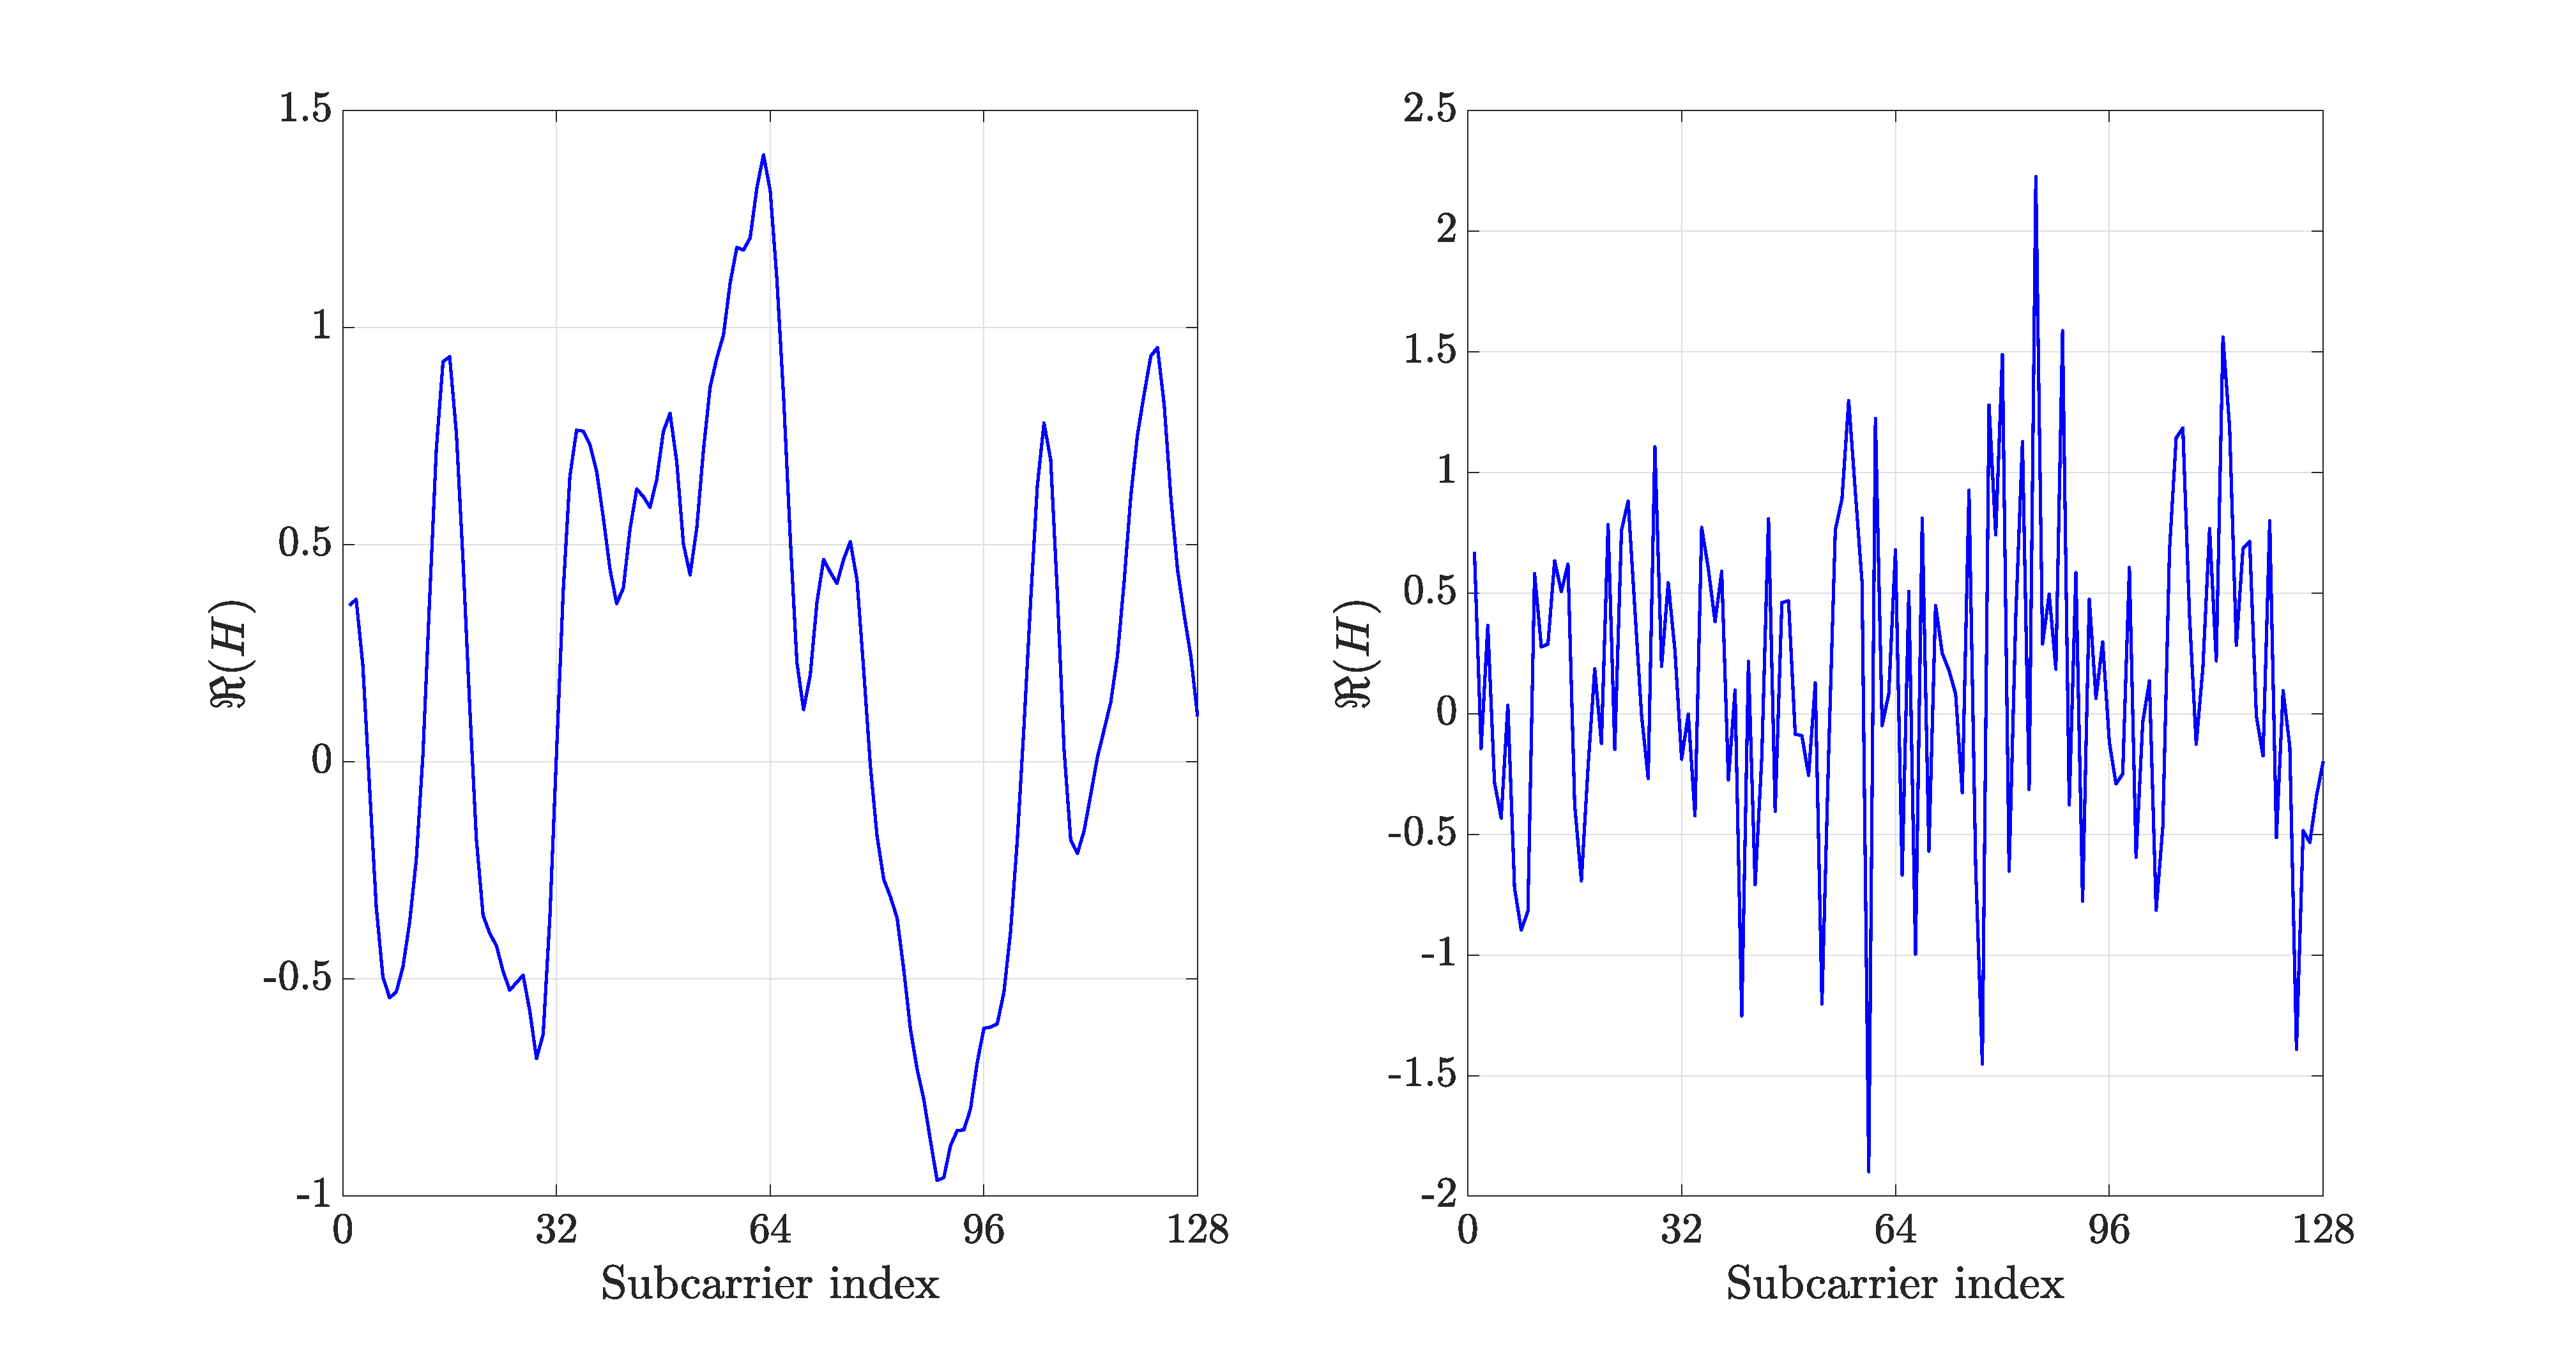
\includegraphics[width=.65\linewidth]{img/channelComparaison.eps}
\caption{Correlated channel ($\beta/N = 1/6$) ; Uncorrelated channel ($\beta/N = 100$)}
\label{fig:channel}
\end{figure} 
In order to generate a correlated channel, we will perform a Choleski decomposition of the correlation matrix. It decomposes a square, symmetric and positive semi-definite matrix into an unique product of a lower triangular matrix and its hermitian, such that:
\begin{equation}
	\textbf{C}_H = \textbf{T T}^H
\end{equation}
where
\begin{equation}
	\textbf{T} = 
	\begin{bmatrix}
	t_{1,1} & 0 & \hdots & 0 \\
	t_{2,1} & t_{2,2} & \hdots & 0 \\
	\vdots & & \ddots & \vdots \\
	t_{Q,1} & t_{Q,2} & \hdots & t_{Q,Q}
	\end{bmatrix}
\end{equation}
The Choleski coefficients can be computed in a recursive way thanks to the Cholski algorithm. So, for a given PDP model and delay spread, we can determine the coefficients of the Choleski matrix The diagonal elements are also positive. Bob correlated channel ($\HB$) will then be the product of the Choleski matrix $\textbf{T}$ with an uncorrelated channel ($\textbf{H}$), i.e., $\HB = \textbf{T H}$. A a consequence, a particular channel component will be a weighted sum depending on the channel components:
\begin{equation}
 	h_{\text{B},j} = \sum_{k = 1}^{j} t_{j,k} h_k
 	\label{eq:corr_channel}
\end{equation}
Note that for an uncorrelated channel, $\textbf{T} = \textbf{I}_Q$ is the identity matrix. In doing so, each subcarrier is independant from the others. We also have:
\begin{equation}
	\sum_{k = 1}^{j} \left| t_{j,k}\right|^2 = 1
	\label{eq:chol_properties}
\end{equation}


%%%%%%%%%%%%%%%%%%%%%%%%%%
\section{SINR Modeling}
In this section, we introduce correlation among Bob's subcarriers only. We consider that Eve channel is uncorrelated. \textcolor{red}{Au début, je pensais intuitivement que ne pas mettre de la corrélation chez Eve était le worst case scénario en terme de sécurité (que ça maximisait la capacité à Eve). Ca s'est avéré ne pas être vrai (cfr plus bas). Mais du coup, je n'ai fait les calculs qu'en considérant de la corrélation à Bob.}. As a reminder, the ergodic SINR is modelized in order to find an approximation of the ergodic capacity using the Jensen's innequality:
\begin{equation}
	\EX{\log_2(1+X)} \leq \log_2(1+\EX{X}) 
	\label{eq:jensen_innequality}
\end{equation}
where $X$ is Bob/Eve SINR. When no correlation was introduced, the innequality bound was tight such that it was used as an approximation. \\
As a reminder, Bob and Eve channels are spatially uncorrelated. 
\subsection{Bob SINR}
At Bob, the received signal is given by:
\begin{equation}
\textbf{y}_{\text{B}}^H = \sqrt{\alpha}\spread^H  \module{\HB}^2\spread\; \textbf{x} +  \spread^H \textbf{v}_\text{B} 
\label{eq:rx_bob}
\end{equation}
The ergodic SINR is then:
\begin{equation}
	\EX{\gamma_B} = \frac{\alpha\EX{\left| \spread^H  \module{\HB}^2\spread\ \right|^2}}{ \EX{\left|  \spread^H \textbf{v}_\text{B}\right|^2}}
	\label{eq:expected_sinrb}
\end{equation}
For a particular symbol $n$, the expected value of the data component is:
\begin{equation}
\begin{split}
\EX{\left| \text{data}\right|^2} &=  \frac{\alpha}{U^2} \EX{\left|\sum_{i=0}^{U-1} \left|h_{B,n+iN}\right|^2\right|^2} \\
&=  \frac{\alpha}{U^2} \EX{\sum_{i=0}^{U-1} \left|h_{B,n+iN}\right|^4  + \sum_{i=0}^{U-1}\sum_{j \neq i}^{U-1} \left|h_{B,n+iN}\right|^2  \left|h_{B,n+jN}\right|^2 }
\label{eq:data_b_determination}
\end{split}
\end{equation}
We can show that:
\begin{equation}
	 \EX{\sum_{i=0}^{U-1} \left|h_{B,n+iN}\right|^4} = 2U
	 \label{eq:data_b_determination_1}
\end{equation}
Also:
\begin{equation}
\begin{split}
\EX{\sum_{i=0}^{U-1}\sum_{j \neq i}^{U-1} \left|h_{B,n+iN}\right|^2  \left|h_{B,n+jN}\right|^2} =& \sum_{i=0}^{U-1} \sum_{j>i}^{U-1} \Bigg(\sum_{k=1}^{n+iN} 2 \module{t_{n+iN,k}}^2   \module{t_{n+jN,k}}^2 + \\
& \sum_{k=1}^{n+iN} \sum_{k'\neq k}^{n+jN} \module{t_{n+iN,k}}^2   \module{t_{n+jN,k'}}^2 +\\
& \sum_{k=1}^{n+iN} \sum_{k'>k}^{n+jN} 2 R [ t_{n+iN,k} t_{n+iN,k'}^* t_{n+jN,k}^* t_{n+jN,k'}] \Bigg)
\label{eq:data_b_determination_2}
\end{split}
\end{equation}
For the noise component: 
\begin{equation}
	\EX{\left| \text{noise}\right|^2} = \sigma^2_{B}
	\label{eq:noise_b_determination}
\end{equation}
The SINR is simply the ratio between eq.(\ref{eq:data_b_determination_2}) and (\ref{eq:noise_b_determination})
\begin{figure}[htb!]
	\centering
	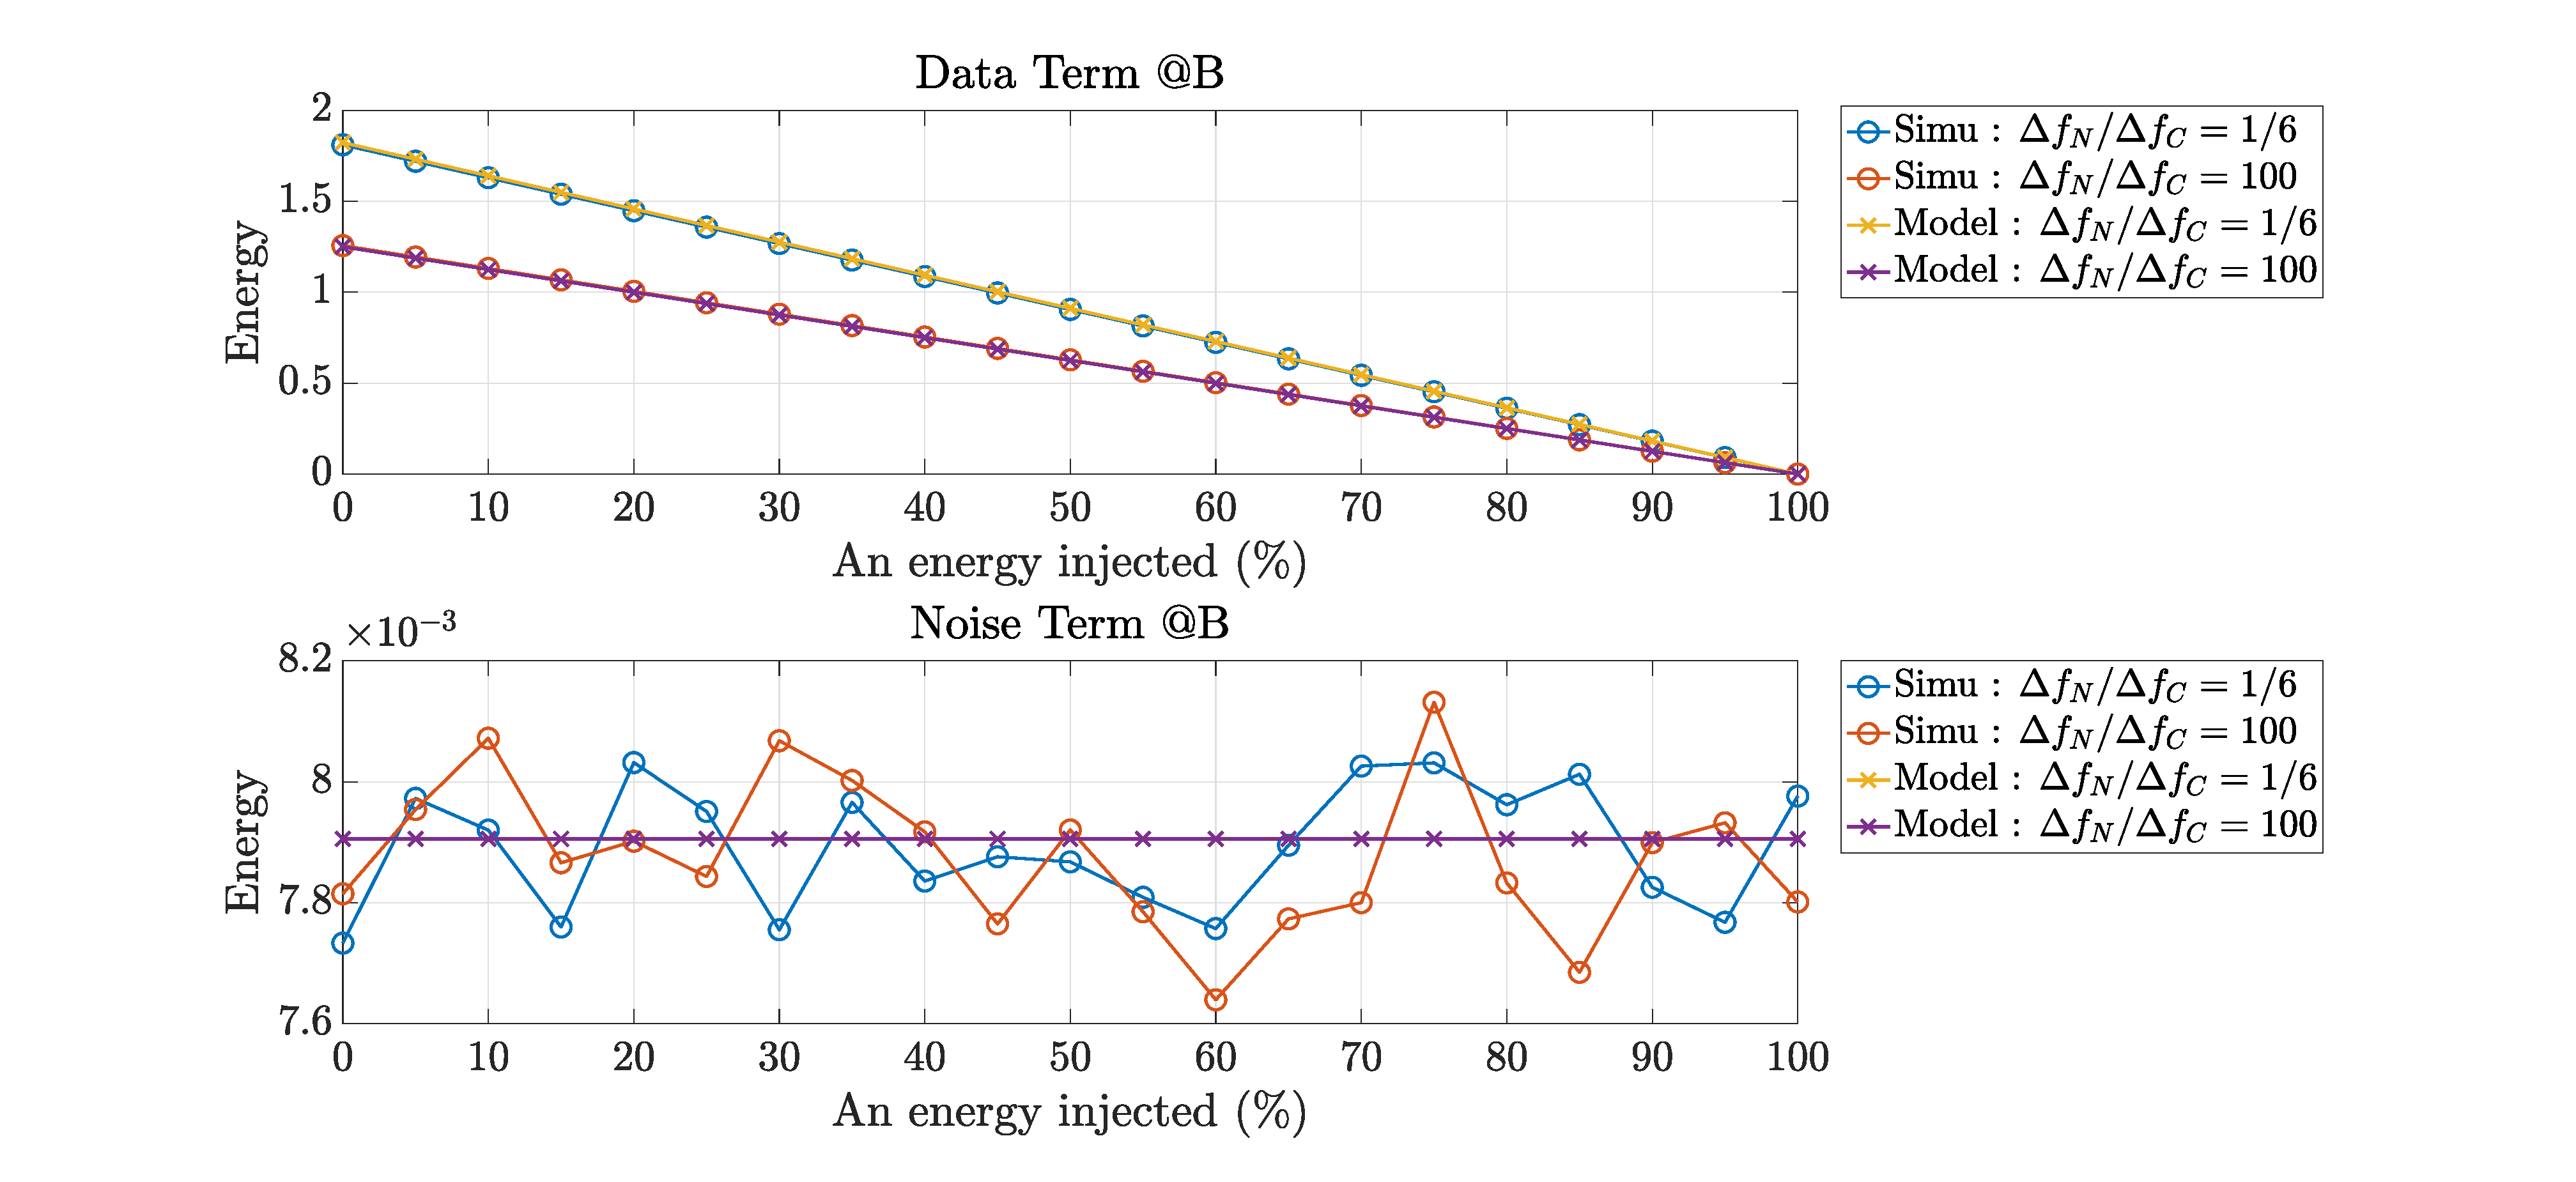
\includegraphics[width=.88\linewidth]{img/bob_sinr_terms_fit.eps}
	\caption{Bob SINR terms fiting, modelization vs simulation}
	\label{fig:SINR_terms_fits}
\end{figure} \\
From Fig.\ref{fig:SINR_terms_fits}, we observe that the analytic expressions (\ref{eq:data_b_determination_2}) and (\ref{eq:noise_b_determination}) well fit the simulation results. In particular, we remark that the received data energy increases when the correlation increases. 


\subsection{Eve SINR}
\paragraph*{SDS Decoding Structure}
When Eve simply despread the received signal, we have
\begin{equation}
\textbf{y}_{\text{E}}^{SDS} = \sqrt{\alpha}\spread^H  \HB^H \HE \spread\; \textbf{x} +  \spread^H \textbf{v}_\text{E} + \sqrt{1-\alpha} \spread^H \HE\textbf{w}
\label{eq:rx_SDS_eve}
\end{equation}
The ergodic SINR is then:
\begin{equation}
\EX{\gamma_E^{SDS}} = \frac{\alpha\EX{\left| \spread^H  \HE\HB^H\spread\ \right|^2}}{ \EX{\left|  \spread^H \textbf{v}_\text{E}\right|^2 + (1-\alpha)  \left| \spread^H  \HE \textbf{w} \right|^2 }} \\
\label{eq:expected_sinr_SDS_e}
\end{equation}
For a particular symbol $n$, the ergodic data component energy is:
\begin{equation}
\begin{split}
\EX{\left| \text{data}\right|^2} &=  \frac{\alpha}{U^2} \EX{\left|\sum_{i=0}^{U-1} h^*_{B,n+iN}h_{E,n+iN}\right|^2} \\
&=  \frac{\alpha}{U^2} \EX{\sum_{i=0}^{U-1} \left|h_{B,n+iN}\right|^2 \left|h_{E,n+iN}\right|^2 + \sum_{i=0}^{U-1}\sum_{j \neq i}^{U-1} h^*_{B,n+iN}  h_{B,n+jN} h_{E,n+iN}  h^*_{E,n+jN} } \\
&= \frac{\alpha}{U^2} \EX{\sum_{i=0}^{U-1} \left|h_{B,n+iN}\right|^2 .1} = \frac{\alpha}{U}
\label{eq:data_E_SDS_determination}
\end{split}
\end{equation}
Eq.(\ref{eq:data_E_SDS_determination}) gives the same result as if no correlation was introduced at Bob. Obviously the AN and noise terms will not depend on Bob correlation. 
For the noise component: 
\begin{equation}
\EX{\left| \text{noise}\right|^2} = \sigma^2_{E}
\label{eq:noise_e_SDS_determination}
\end{equation}
For the AN component:
\begin{equation}
\EX{\left| \text{AN}\right|^2} = \frac{(1-\alpha)}{U} \sigma_{AN}^2 = (1-\alpha)
\label{eq:noise_an_SDS_determination}
\end{equation}
The SINR is therefore identical as in the case where Bob channel is uncorrelated.\\

\textcolor{red}{Je ne montre pas les calculs pour le matched filter ni le own channel decoder parce que le problème qui suit aparaît déjà pour la capacité à Bob. Mais, les mêmes soucis apparaissent aussi pour les structures de décodage à Eve.}

%%%%%%%%%%%%%%%%%%%%%%%%%%
\section{Jensen's innequality issue}
In the past works, the Jensen innequality was used as a good approximation when no correlation was introduced among Bob's subcarriers. When the correlation is introduced, the approximation does not hold anymore, as seen in Fig(\ref{fig:capaB_ergo_jensen}). In particular, we observe that, when $\Delta f_N / \Delta f_C = 100$, i.e., uncorrelated channel, the fit between analytic and simulation curves is almost perfect. However, when $\Delta f_N / \Delta f_C = 1/6$, i.e., highly correlated channel, the ergodic capacity decreases but the approximation suggests that it should increase. 
\begin{figure}[htb!]
	\centering
	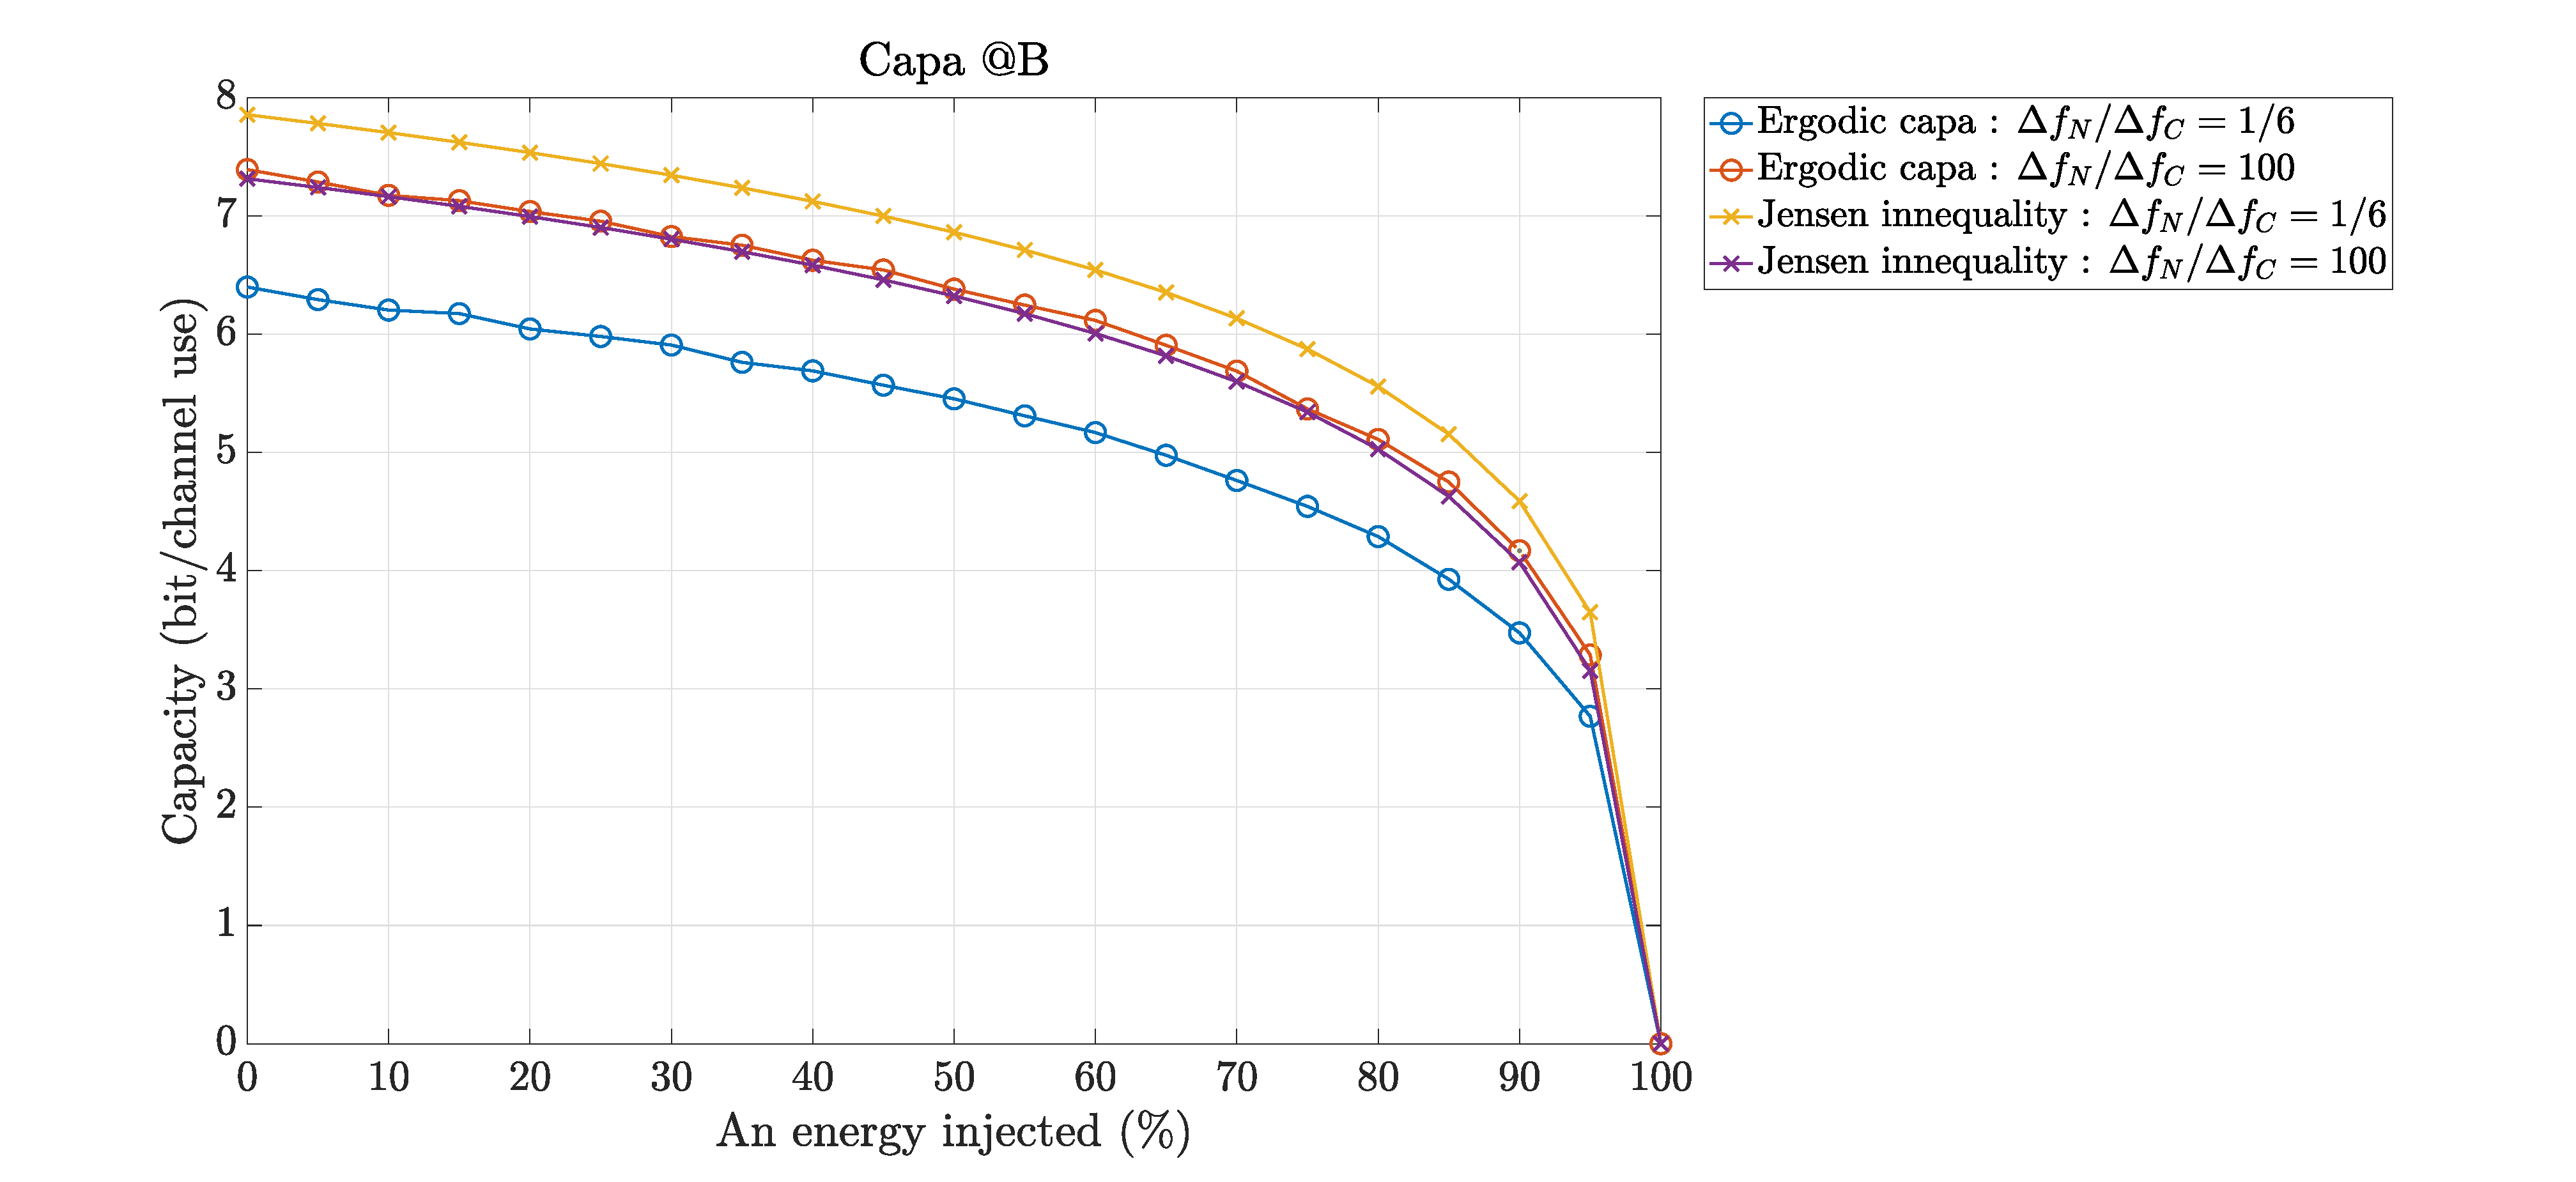
\includegraphics[width=.75\linewidth]{img/capaB_ergoVSjensen.eps}
	\caption{Bob capacity, variable correlation, ergodic vs Jensen's innequality}
	\label{fig:capaB_ergo_jensen}
\end{figure} 
In order to understand the behaviour of the analytic model of the capacity derived using the Jensen's innequality as an approximation, we will analyze eq.(\ref{eq:data_b_determination}). When Bob's channel is fully correlated, i.e., all subcarriers are an identical complex scalar, $h_{B,n+iN} = h_{B,n+jN}, \; \forall i,j$. Therefore, eq.(\ref{eq:data_b_determination}) becomes:
\begin{equation}
\begin{split}
\EX{\left| \text{data}\right|^2} &=  \frac{\alpha}{U^2} \EX{\left|\sum_{i=0}^{U-1} \left|h_{B,n+iN}\right|^2\right|^2} \\
&=  \frac{\alpha}{U^2} \EX{\sum_{i=0}^{U-1} \left|h_{B,n+iN}\right|^4  + \sum_{i=0}^{U-1}\sum_{j \neq i}^{U-1} \left|h_{B,n+iN}\right|^2  \left|h_{B,n+jN}\right|^2 } \\
&=  \frac{\alpha}{U^2} \left(2U + 2U(U-1) \right)= 2\alpha
\label{eq:data_b_determination_fullCorrel}
\end{split}
\end{equation}
When Bob's channel is totally uncorrelated, eq.(\ref{eq:data_b_determination}) becomes:
\begin{equation}
\begin{split}
\EX{\left| \text{data}\right|^2} &=  \frac{\alpha}{U^2} \EX{\left|\sum_{i=0}^{U-1} \left|h_{B,n+iN}\right|^2\right|^2} \\
&=  \frac{\alpha}{U^2} \EX{\sum_{i=0}^{U-1} \left|h_{B,n+iN}\right|^4  + \sum_{i=0}^{U-1}\sum_{j \neq i}^{U-1} \left|h_{B,n+iN}\right|^2  \left|h_{B,n+jN}\right|^2 } \\
&=  \frac{\alpha}{U^2} \left(2U + U(U-1) \right)= \frac{\alpha(U+1)}{U}
\label{eq:data_b_determination_noCorrel}
\end{split}
\end{equation}
Eq.(\ref{eq:data_b_determination_fullCorrel}) and (\ref{eq:data_b_determination_noCorrel}) suggest that Bob ergodic SINR increases when the correlation increases:
\begin{equation}
	\frac{\alpha(U+1)}{U \sigma_B^2}\Bigg|_{\text{no correl}} \leq \EX{\gamma_B} \leq \frac{2\alpha}{\sigma_B^2}\Bigg|_{\text{full correl}}
\end{equation}
This behaviour can be seen in Fig.(\ref{fig:sinr_capa_variableCorrelB}). This implies that the approximated capacity $\log_2{(1+\EX{\gamma_B})}$ should increase with an increase of the correlation. However, it is observed in Fig.(\ref{fig:sinr_capa_variableCorrelB}) that the ergodic capacity $\EX{\log_2{(1+\gamma_B)}}$ decreases with an increase of the correlation.
\begin{figure}[htb!]
	\centering
	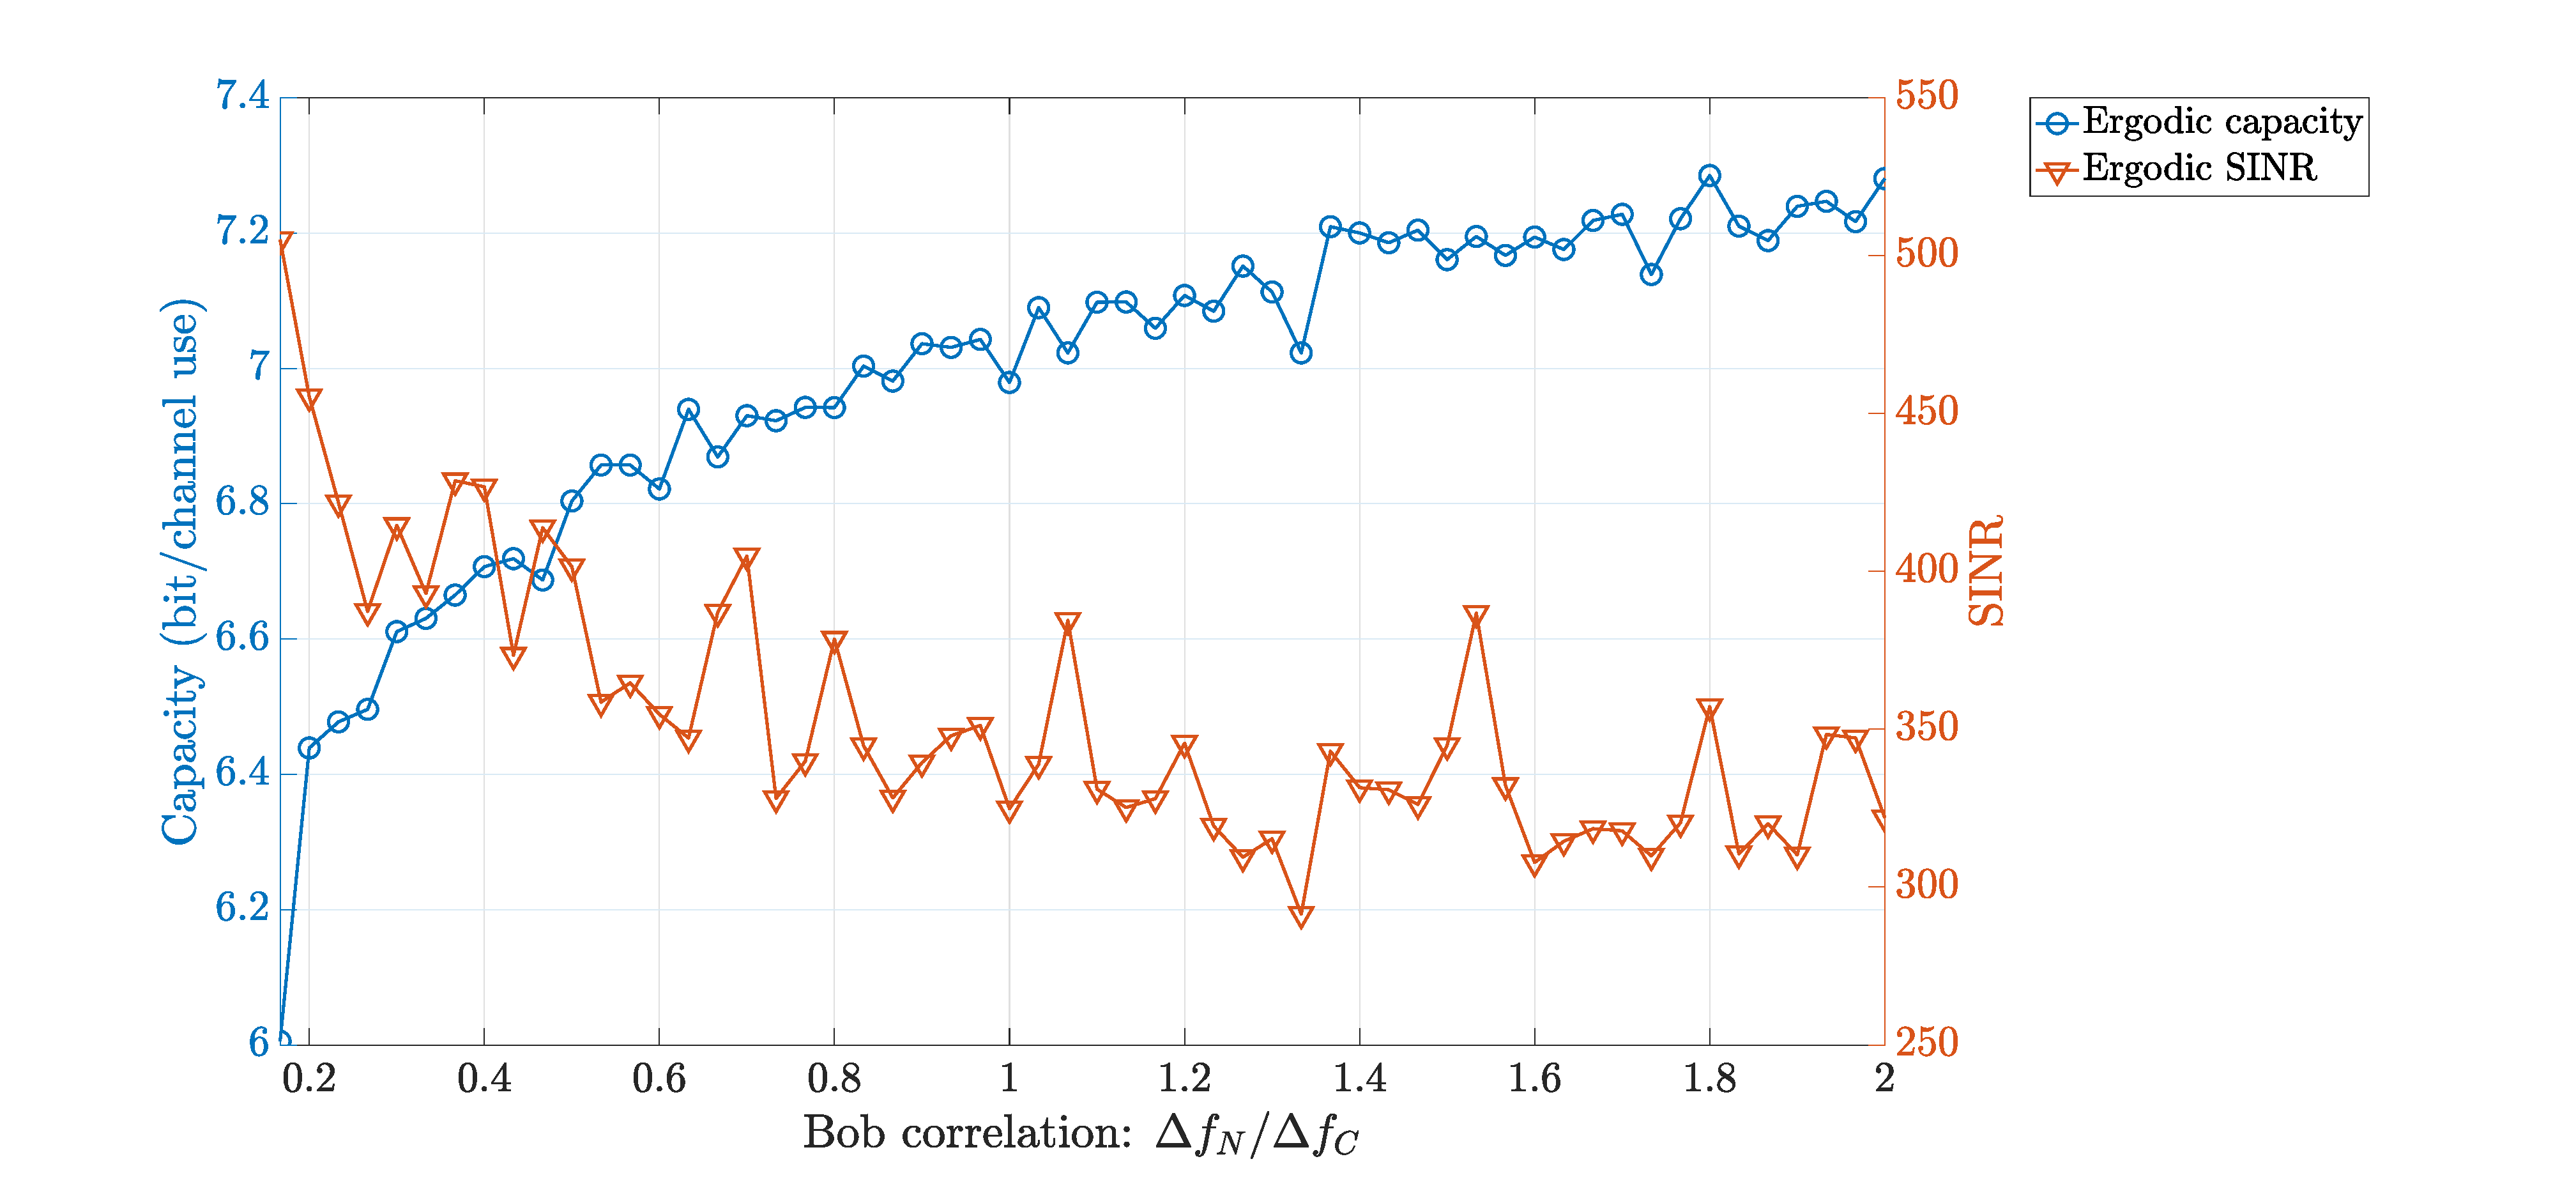
\includegraphics[width=.75\linewidth]{img/SINR_capa_variableCorrelB.eps}
	\caption{Bob SINR/capacity as a function of the frequency  correlation}
	\label{fig:sinr_capa_variableCorrelB}
\end{figure}\\
\textcolor{red}{Je ne sais pas expliquer pourquoi l'ergodic capacité se comporte différemment que l'ergodic SINR... Any idea? J'ai lu qu'on pouvait peut-être estimer l'erreur provoquée par Jensen en calculant le \textit{Jensen's gap}. Mais ça ne m'a pas l'air trivial du tout...}\\
Another approximation of the capacity is therefore needed.





%%%%%%%%%%%%%%%%%%%%%%%%%%
\section{Second order Taylor approximation of the capacity}
In order to better approximate the ergodic capacity, it was decided to  perform a second order Taylor expansion of $\EX{\log_2{(1+\gamma)}}$ around $x_0 = \EX{\gamma}$, where $\gamma$ represents Bob or Eve SINR, depending on the investigated scenario:
\begin{equation}
	\EX{\log_2(1+\gamma)} \approx \log_2(1+\EX{\gamma}) - \frac{\text{var}(\gamma)}{2(1+\EX{\gamma})^2}
	\label{eq:second_order_approx}
\end{equation}
where $\text{var}(\gamma) = \EX{\gamma^2} - \left(\EX{\gamma}\right)^2$ is the SINR variance, which is quite complicated to derive.\\
\textcolor{red}{Auriez-vous une idée pour une meilleure approximation?}




\paragraph*{Bob variance derivation}
The terme $\EX{\gamma_B^2}$ is difficult to derive. In fact:
\begin{equation}
	\EX{\gamma_B^2} = \left( \frac{\alpha\EX{\left| \spread^H  \module{\HB}^2\spread\ \right|^2}}{ \EX{\left|  \spread^H \textbf{v}_\text{B}\right|^2}}\right)^2 = \frac{\alpha^2 \EX{\left| \spread^H  \module{\HB}^2\spread\ \right|^4}}{\EX{\left|  \spread^H \textbf{v}_\text{B}\right|^4}}
	\label{eq:sinrB_exp4}
\end{equation} 
Since $v_B \sim \mathbb{C}N(0,\sigma_B^2) \sim N(0,\sigma_B^2/2) + 1j N(0,\sigma_B^2/2)$, it is easy to show that \footnote{\textcolor{red}{Personnal note: cfr FC17 verso for the derivation}}:
\begin{equation}
	\EX{\left|  \spread^H \textbf{v}_\text{B}\right|^4} = 2(\sigma_B^2)^2
	\label{eq:noisB_exp4}
\end{equation}
In what concerns the data term, for a particular symbol $n$, the derivation is quite long:
\begin{equation}
\begin{split}
	\EX{\module{\text{data}}^4} = &\frac{\alpha^2}{U^4} \mathbb{E}\Bigg[ \module{\sum_{i=0}^{U-1}\module{h_{B,n+iN}}^2}^4\Bigg] \\
	= &\frac{\alpha^2}{U^4} \mathbb{E}\Bigg[ \sum_{i=0}^{U-1} \module{h_{B,n+iN}}^8 + 4 \sum_{i=0}^{U-1} \sum_{j \neq i}^{U-1} \module{h_{B,n+iN}}^2\module{h_{B,n+jN}}^6 \\
	& + 3 \sum_{i=0}^{U-1} \sum_{j \neq i}^{U-1} \module{h_{B,n+iN}}^4\module{h_{B,n+jN}}^4 + 6 \sum_{i=0}^{U-1} \sum_{j \neq i}^{U-1} \sum_{k \neq i,j}^{U-1} \module{h_{B,n+iN}}^4\module{h_{B,n+jN}}^2  \module{h_{B,n+kN}}^2 \\ 
	& + \sum_{i=0}^{U-1} \sum_{j \neq i}^{U-1} \sum_{k \neq i,j}^{U-1}   \sum_{l \neq i,j,k}^{U-1} \module{h_{B,n+iN}}^2\module{h_{B,n+jN}}^2  \module{h_{B,n+kN}}^2   \module{h_{B,n+lN}}^2\Bigg] 
\end{split}
\label{eq:dataB_exp4}
\end{equation}
Knowing that:
\begin{equation}
	\begin{split}
		&\EX{h_{B,i} h_{B,j} } \neq 0 \\
		& h_{B,n+iN} = \sum_{k = 1}^{n+iN} t_{n+iN,k} h_k
	\end{split}
\end{equation}
the resolution of eq(\ref{eq:dataB_exp4}) is tedious. \textcolor{red}{Par exemple le second terme en $h^2 h^6$ donne lieu à 10 termes à calculer. Chacun de ces 10 termes correspond à plusieurs lignes de calcul. Le dernier terme de (31) en $h^2h^2h^2h^2$ donne lieu au calcul de 6 termes, dont un fait 13 lignes de calculs... Néanmoins je les ai tous calculé et verifié un par un. Si tout est décorrélé, ce calcul est très simple car à ce moment l'expected value d'un produit est égal au produit des expected values. Il faut juste savoir que: $\EX{\module{h}^2} = 1$, $\EX{\module{h}^4} = 2$, $\EX{\module{h}^6} = 6$ et $\EX{\module{h}^8} = 24$. Après, je me rends compte que le calcul est ultra simple aussi dans le cas \textit{full correlated}. Dans le sens où on aurait plus que du $\EX{\module{h}^8}$ pour tous les termes car $h_{B,n+iN} = h_{B,n+jN}, \forall i,j$. Peut-être qu'alors l'approximation serait meilleure??? (voir la suite pour comprendre que l'approximation n'est pas top). Est-ce que vous désirez les calculs complets??}

\paragraph*{Eve SDS decoder variance}
Also derived but less complicated since:
\begin{equation}
\begin{split}
\EX{\module{\text{data}}^4} = &\frac{\alpha^2}{U^4} \mathbb{E}\Bigg[ \module{\sum_{i=0}^{U-1}h^*_{B,n+iN} h_{E,n+iN}}^4\Bigg] \\
= &\frac{\alpha^2}{U^4} \mathbb{E}\Bigg[ \sum_{i=0}^{U-1} \module{h_{B,n+iN}}^4   \module{h_{E,n+iN}}^4  +2 \sum_{i=0}^{U-1} \sum_{j \neq i}^{U-1} \module{h_{B,n+iN}}^2\module{h_{B,n+jN}}^2\module{h_{E,n+iN}}^2 \module{h_{E,n+jN}}^2 \Bigg] \\
=& \frac{2\alpha^2}{U^4}   \mathbb{E}\Bigg[\sum_{i=0}^{U-1} \module{h_{B,n+iN}}^4  + \sum_{i=0}^{U-1} \sum_{j \neq i}^{U-1} \module{h_{B,n+iN}}^2\module{h_{B,n+jN}}^2  \Bigg] 
\end{split}
\label{eq:dataE_exp4}
\end{equation}



\section{Results}
\paragraph*{Approximation accuracy comparison}


\begin{figure}[htb!]
	\centering
	\includegraphics[width=.67\linewidth]{img/comparaisonApprox_highCorrel_16Q8U.eps}
\caption{High correlation, $Q=16$, $U=8$, approximation comparaison}
	\label{fig:approxComparaison}
\end{figure}
\begin{figure}[htb!]
	\centering
	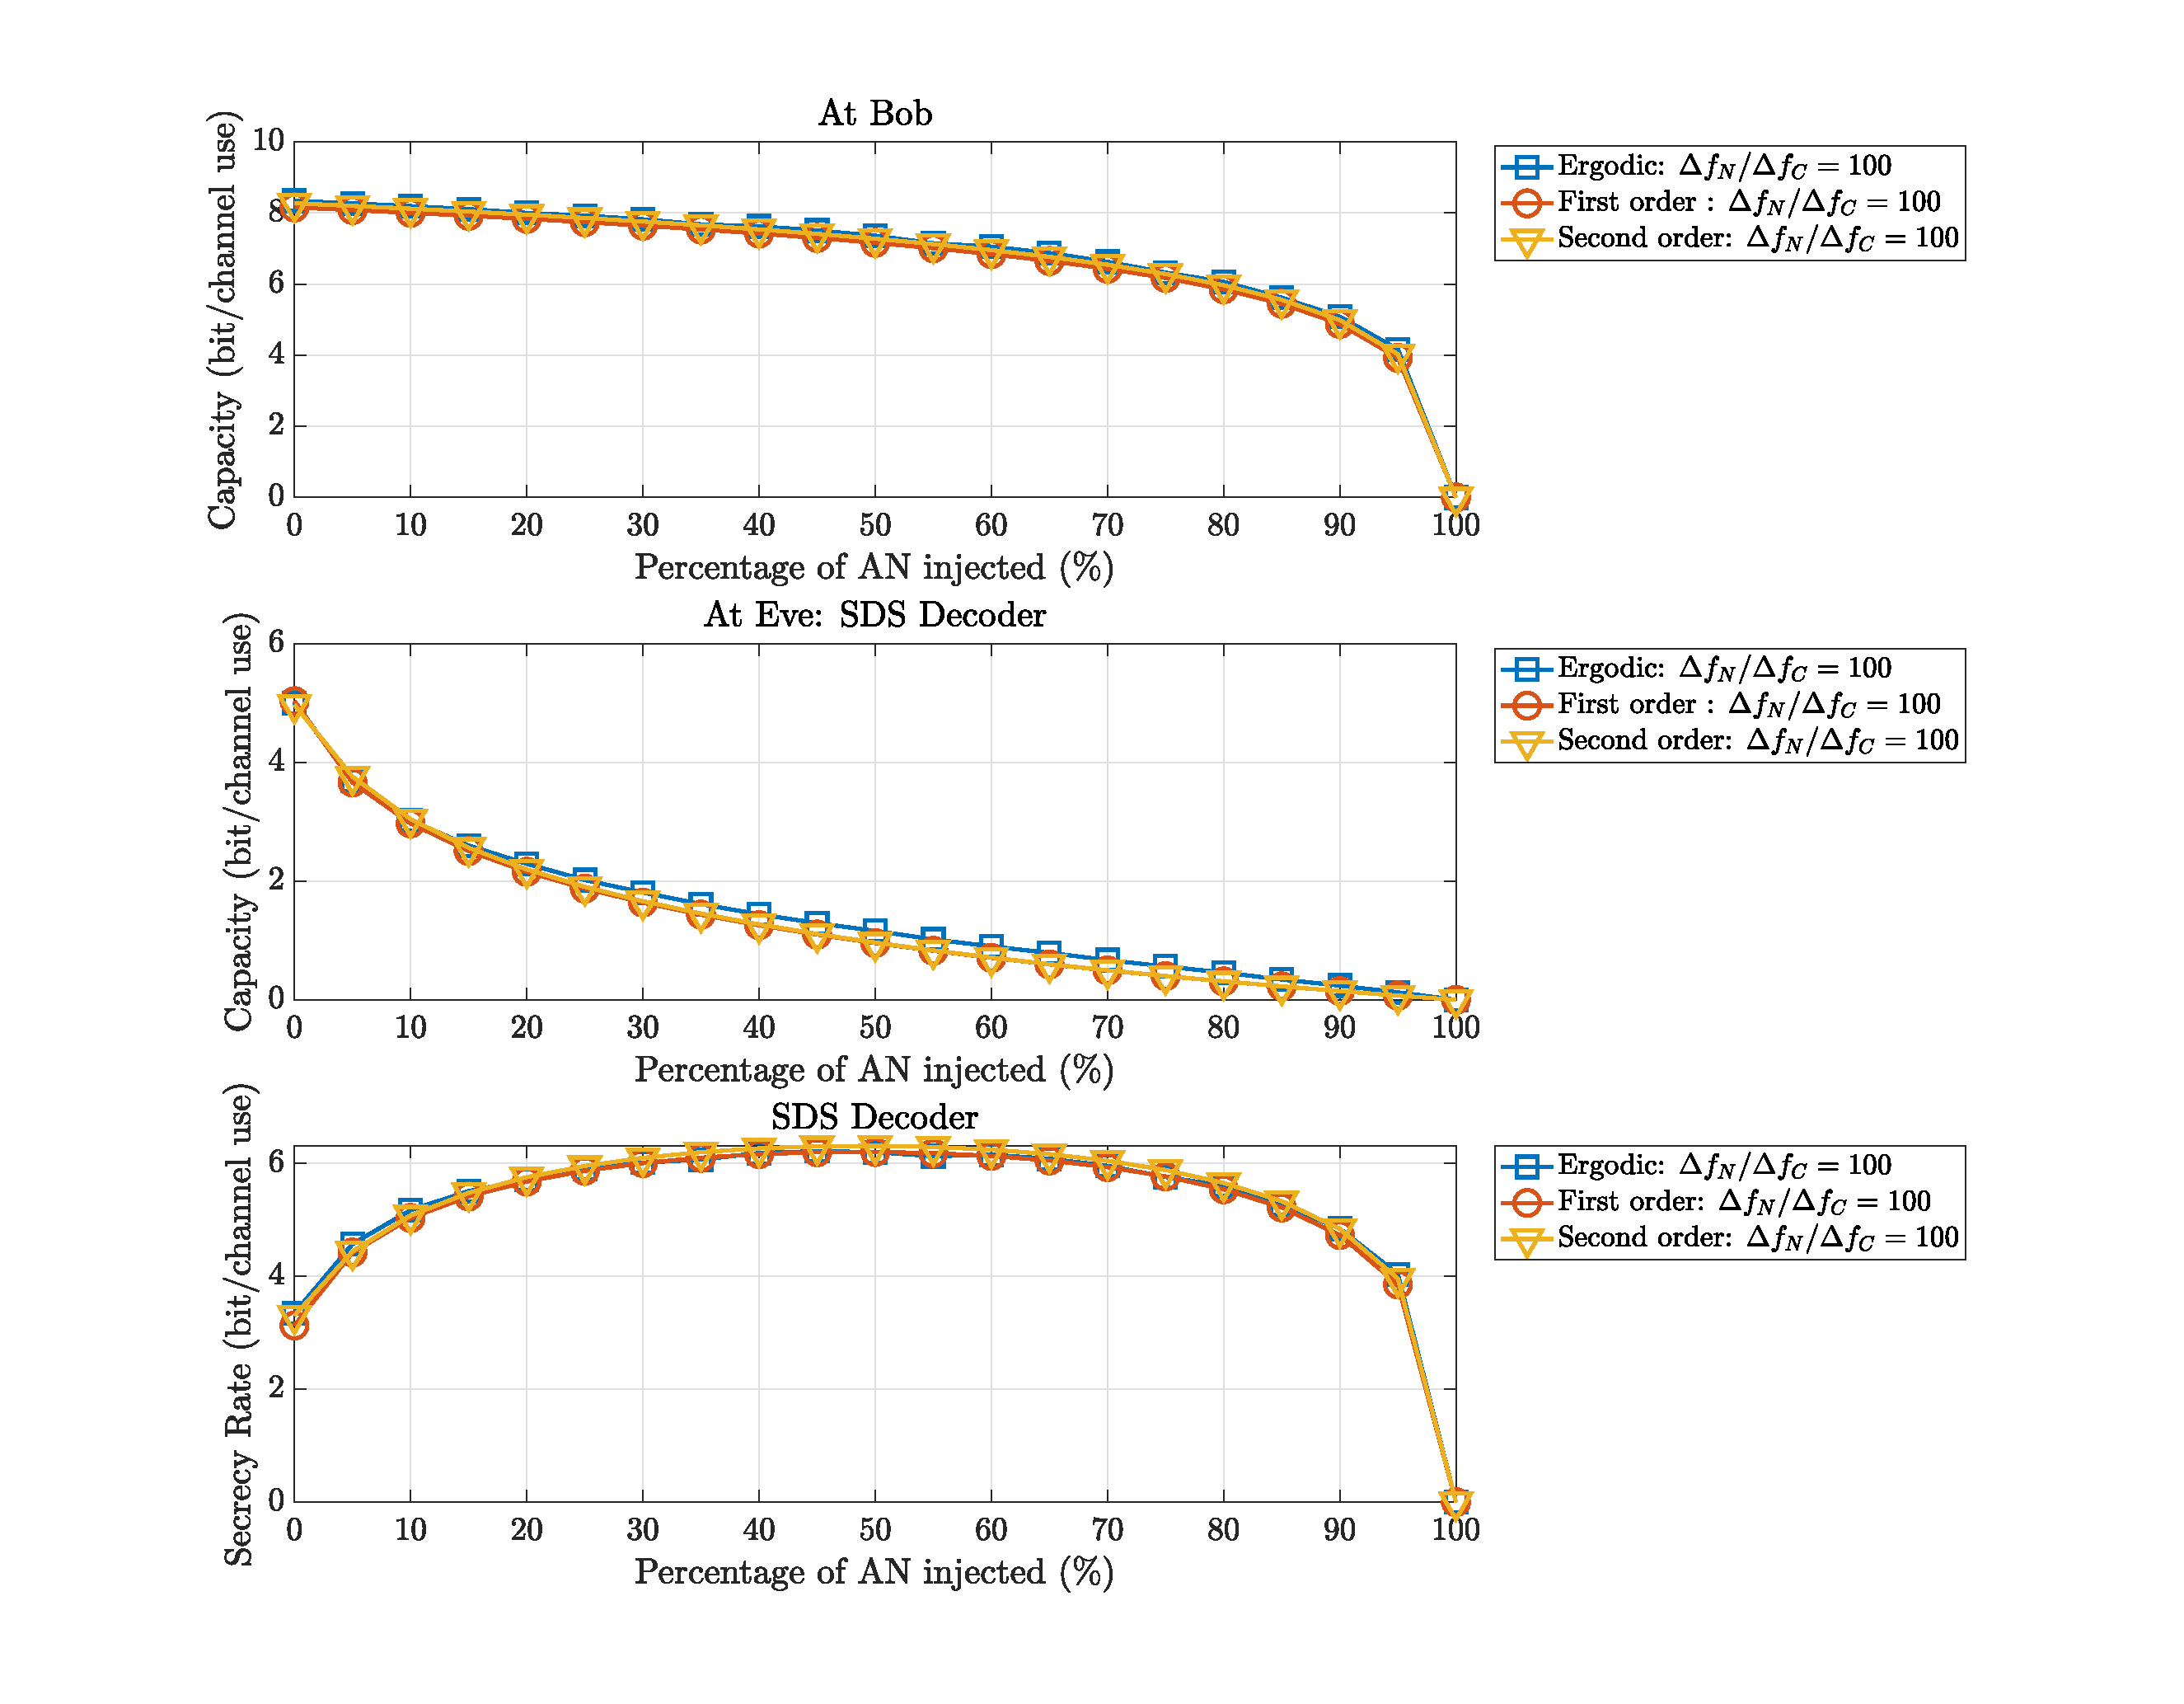
\includegraphics[width=.67\linewidth]{img/comparaisonApprox_noCorrel_16Q8U.eps}
	\caption{No correlation,  $Q=16$, $U=8$, approximation comparaisons}
	\label{fig:approxComparaison2}
\end{figure}
Fig\ref{fig:approxComparaison} and \ref{fig:approxComparaison2} compare the accuracy of the two approximations (first order using Jensen, second order using Jensen plus the variance term) with the ergodic results, for 2 different environments, i.e., high correlation (fig\ref{fig:approxComparaison}) and low correlation (fig\ref{fig:approxComparaison2}). \\

As expected, when no correlation is introduced, the first order approximation approximates well the ergodic curves. There is no need to use another approximation.  We also observe that the second order approximation is better than the first order approximation when the correlaton is introduced. However, the SR bound is not tight. Furthermore, it is an upper bound when we would be happier with a lower one in order to a priori know at least the rate at which to securely communicate. \\

What is interesting though, is that the SR curves present the same concavity. In particular, the analytic determination of the optimal amount of data to inject (optimal $\alpha$) can be accurately found using the first order approximation \textcolor{red}{(I did it)}.\\

Fig.\ref{fig:maxSR1_approxComparaison} shows the maximal SR value as a function of the amount of correlation at Bob. We observe that the first order approximation increases with an increase of the correlation, as already explained. The second order remains quasi constant. 
\begin{figure}[htb!]
	\centering
	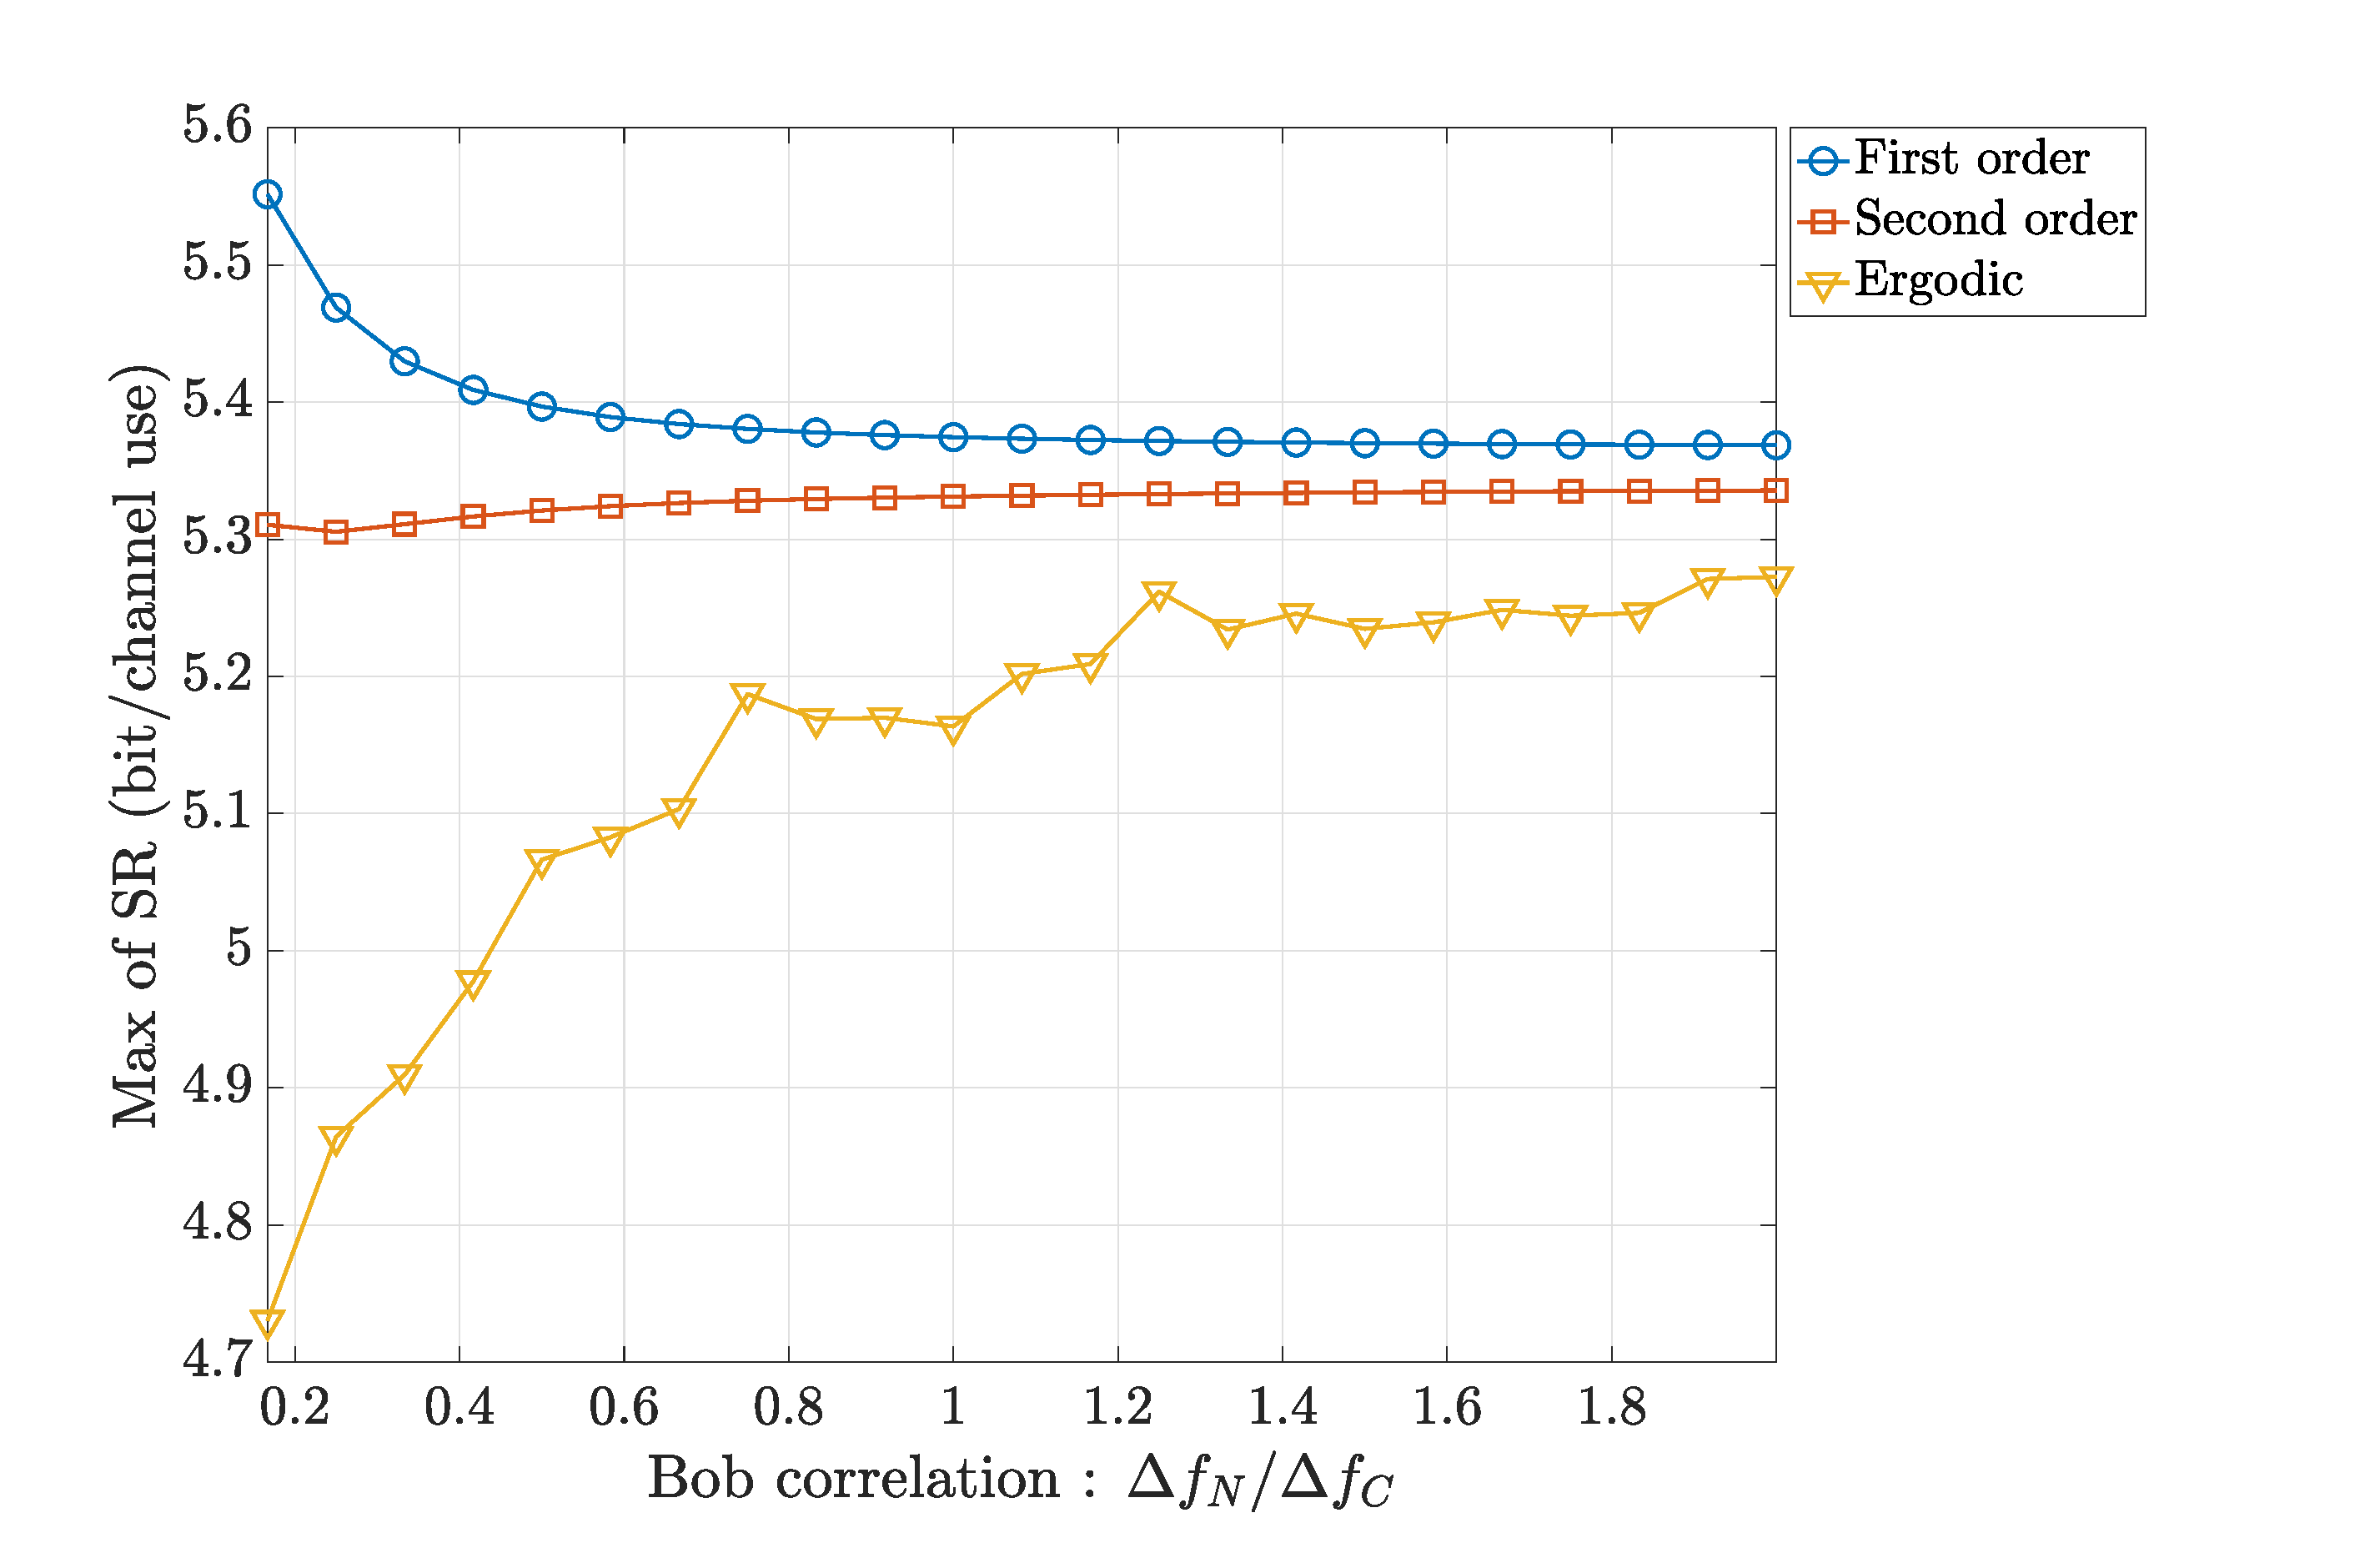
\includegraphics[width=.7\linewidth]{img/maxSR1_noCorrelE_variableB_approx_Q32U4.eps}
	\caption{Maximum of SR, SDS Decoder at Eve, variable correlation at Bob, $Q=32$, $U=4$, approximation comparaison}
	\label{fig:maxSR1_approxComparaison}
\end{figure}\\

\textcolor{red}{Ici, les questions suivantes se posent:
\begin{itemize}
	\item L'approximation du second est-elle utilisable?
	\item Y'a t'il une autre approximation qui pourrait être utilisée?
\end{itemize}}






\paragraph*{Other obtained results}
\begin{itemize}
	\item Determination of the optimal $\alpha$ to maximize the ergodic SR
	\item First and second order approximations for Eve matched filter and own channel decoders
	\item Required SNR at Bob in order to guarantee a given SR, i.e. SNR$= \infty$ at Eve. No analytic expression, only via simulations since the analytic approximations are not tight enough.
	\item Simulations (no analytic model yet) with variable correlation among Eve's subcarriers, i.e., influence of Eve correlation on the performances. It seem that introducing correlatin at Eve decreases the SR performances
\end{itemize}

\textcolor{red}{\textbf{POUR CONCLURE:\\
Je suis un peu embêté car je ne sais pas trop comment valoriser ces résultats. Est-ce que tout étudier via des simulations seulement est intéressant? Dans le sens où les formules dérivées ne sont pas terribles. Ca sera un peu bête de tout jeter...}}









\end{document}
